\begin{itemize}

    \item Một miền cần chia đủ nhỏ để phù hợp với một nhóm cụ thể. Để đạt được điều này, chúng ta cần xác định rõ ranh giới giữa các ngữ cảnh.
    
    \item Bối cảnh giới hạn (Bounded Context) giúp định rõ các ranh giới, chia miền thành các phần độc lập để giải quyết sự phức tạp trong mô hình doanh nghiệp.
    
    \item Bối cảnh giới hạn thể hiện phạm vi kinh doanh của dịch vụ.
    
    \item Bối cảnh giới hạn tạo ra các mô hình khác nhau cho các lĩnh vực khác nhau của miền.
    
    \item Bối cảnh giới hạn tương ứng với một nhóm cụ thể trong tổ chức.
    
    \end{itemize}
    
    \begin{figure}[H]
    
    \centering
    
    % 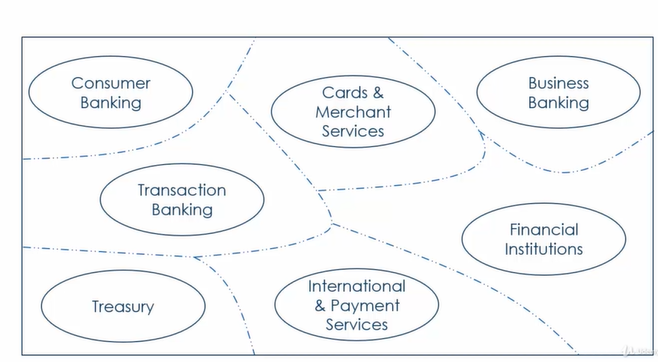
\includegraphics[width = 0.8\textwidth]{pictures/boi_canh_gioi_han/main.png}
    
    \caption{Ví dụ về bối cảnh giới hạn trong một ngân hàng}
    
    \end{figure}
    
    \subsubsection{Một vài hướng xác định bối cảnh giới hạn}
    
    \begin{itemize}
    
    \item Việc xác định bối cảnh giới hạn được điều chỉnh bởi sự gắn kết giữa các miền phụ.
    
    \item Dựa vào sơ đồ cấu trúc tổ chức các phòng ban của doanh nghiệp.
    
    \item Dựa vào modules của các ứng dụng kiến trúc nguyên khối (nếu việc phân chia tốt).
    
    \item Dựa vào trách nhiệm và hoạt động của chuyên gia ngành.
    
    \end{itemize}
    
    \end{document}
    
    %!<! - - Hướng dẫn 5/10 - - >